%===============================================================================
% LaTeX sjabloon voor de bachelorproef toegepaste informatica aan HOGENT
% Meer info op https://github.com/HoGentTIN/latex-hogent-report
%===============================================================================

\documentclass[dutch,dit,thesis]{hogentreport}

% TODO:
% - If necessary, replace the option `dit`' with your own department!
%   Valid entries are dbo, dbt, dgz, dit, dlo, dog, dsa, soa
% - If you write your thesis in English (remark: only possible after getting
%   explicit approval!), remove the option "dutch," or replace with "english".

\usepackage{lipsum} % For blind text, can be removed after adding actual content
\usepackage{float}
\restylefloat{table}

%% Pictures to include in the text can be put in the graphics/ folder
\graphicspath{{graphics/}}

%% For source code highlighting, requires pygments to be installed
%% Compile with the -shell-escape flag!
\usepackage[section]{minted}
\usemintedstyle{solarized-light}
\definecolor{bg}{RGB}{253,246,227} %% Set the background color of the codeframe

%% Change this line to edit the line numbering style:
\renewcommand{\theFancyVerbLine}{\ttfamily\scriptsize\arabic{FancyVerbLine}}

%% Macro definition to load external java source files with \javacode{filename}:
\newmintedfile[javacode]{java}{
    bgcolor=bg,
    fontfamily=tt,
    linenos=true,
    numberblanklines=true,
    numbersep=5pt,
    gobble=0,
    framesep=2mm,
    funcnamehighlighting=true,
    tabsize=4,
    obeytabs=false,
    breaklines=true,
    mathescape=false
    samepage=false,
    showspaces=false,
    showtabs =false,
    texcl=false,
}

% Other packages not already included can be imported here

%%---------- Document metadata -------------------------------------------------
\author{Michiel Van Herreweghe}
\supervisor{Mevr. M. Van Audenrode}
\cosupervisor{Dhr. K. Van Moorter}
\title[Optionele ondertitel]%
    {Een onderzoek naar de maturiteit van .NET MAUI bij het vervangen van een real-time POS-systeem}
\academicyear{\advance\year by -1 \the\year--\advance\year by 1 \the\year}
\examperiod{1}
\degreesought{\IfLanguageName{dutch}{Professionele bachelor in de toegepaste informatica}{Bachelor of applied computer science}}
\partialthesis{false} %% To display 'in partial fulfilment'
%\institution{Internshipcompany BVBA.}

%% Add global exceptions to the hyphenation here
\hyphenation{back-slash}

%% The bibliography (style and settings are  found in hogentthesis.cls)
\addbibresource{VanHerrewegheMichiel_BP.bib}            %% Bibliography file
\addbibresource{../1. Voorstel/VanHerrewegheMichiel-BachelorProefVoorstel.bib} %% Bibliography research proposal
\defbibheading{bibempty}{}

%% Prevent empty pages for right-handed chapter starts in twoside mode
\renewcommand{\cleardoublepage}{\clearpage}

\renewcommand{\arraystretch}{1.2}

%% Content starts here.
\begin{document}

%---------- Front matter -------------------------------------------------------

\frontmatter

\hypersetup{pageanchor=false} %% Disable page numbering references
%% Render a Dutch outer title page if the main language is English
\IfLanguageName{english}{%
    %% If necessary, information can be changed here
    \degreesought{Professionele Bachelor toegepaste informatica}%
    \begin{otherlanguage}{dutch}%
       \maketitle%
    \end{otherlanguage}%
}{}

%% Generates title page content
\maketitle
\hypersetup{pageanchor=true}

%%=============================================================================
%% Voorwoord
%%=============================================================================

\chapter*{\IfLanguageName{dutch}{Woord vooraf}{Preface}}%
\label{ch:voorwoord}

%% TODO:
%% Het voorwoord is het enige deel van de bachelorproef waar je vanuit je
%% eigen standpunt (``ik-vorm'') mag schrijven. Je kan hier bv. motiveren
%% waarom jij het onderwerp wil bespreken.
%% Vergeet ook niet te bedanken wie je geholpen/gesteund/... heeft

.NET MAUI is het nieuwste project van Microsoft dat ons toelaat om cross-platform applicaties te ontwikkelen met C\# en .NET. 

Ikzelf ben altijd graag bezig met het uitproberen van nieuwe tools, programmeertalen en features. Dit onderzoek is mij dan ook op het lijf geschreven.

Eerst en vooral wil ik mijn co-promoter \textbf{Kristof Van Moorter} bedanken. Kristof heeft mij met raad en daad bijgestaan op de momenten dat ik het nodig had. Daarnaast wil ik mijn promotoren \textbf{Martine van Audenrode} en \textbf{Chantal Teerlinck} bedanken die altijd de gepaste feedback gaven wanneer ik het vroeg. Ook wil ik heel graag mijn ouders, \textbf{Mario Van Herreweghe} en \textbf{Sabrina Timmermans}, bedanken die mij alle kansen gegeven hebben en mij gevormd hebben tot wie ik nu ben. Verder wil ik ook mijn vriendin \textbf{Ilke Kestemont} bedanken voor alle hulp en ondersteuning die zij mij geboden heeft tijdens het onderzoeken en schrijven van deze bachelorproef.

Tot slot wil ik deze bachelorproef ook opdragen aan mijn peter \textbf{Filip Timmermans}, die er niet meer is. Hij zal mij nooit zien afstuderen, maar op deze manier is hij er toch bij.
%%=============================================================================
%% Samenvatting
%%=============================================================================

% TODO: De "abstract" of samenvatting is een kernachtige (~ 1 blz. voor een
% thesis) synthese van het document.
%
% Een goede abstract biedt een kernachtig antwoord op volgende vragen:
%
% 1. Waarover gaat de bachelorproef?
% 2. Waarom heb je er over geschreven?
% 3. Hoe heb je het onderzoek uitgevoerd?
% 4. Wat waren de resultaten? Wat blijkt uit je onderzoek?
% 5. Wat betekenen je resultaten? Wat is de relevantie voor het werkveld?
%
% Daarom bestaat een abstract uit volgende componenten:
%
% - inleiding + kaderen thema
% - probleemstelling
% - (centrale) onderzoeksvraag
% - onderzoeksdoelstelling
% - methodologie
% - resultaten (beperk tot de belangrijkste, relevant voor de onderzoeksvraag)
% - conclusies, aanbevelingen, beperkingen
%
% LET OP! Een samenvatting is GEEN voorwoord!

%%---------- Nederlandse samenvatting -----------------------------------------
%
% TODO: Als je je bachelorproef in het Engels schrijft, moet je eerst een
% Nederlandse samenvatting invoegen. Haal daarvoor onderstaande code uit
% commentaar.
% Wie zijn bachelorproef in het Nederlands schrijft, kan dit negeren, de inhoud
% wordt niet in het document ingevoegd.

\IfLanguageName{english}{%
\selectlanguage{dutch}
\chapter*{Samenvatting}
\lipsum[1-4]
\selectlanguage{english}
}{}

%%---------- Samenvatting -----------------------------------------------------
% De samenvatting in de hoofdtaal van het document

\chapter*{\IfLanguageName{dutch}{Samenvatting}{Abstract}}

.NET MAUI (Multi-platform App UI) is een nieuw framework voor de ontwikkeling van cross-platform toepassingen die ingezet kan worden voor zowel de desktop als mobiele platformen. Het is ontwikkeld door Microsoft en komt voort uit het eerdere Xamarin.Forms framework. Met NET MAUI kunnen ontwikkelaars een enkele codebase schrijven en delen op verschillende platforms, waaronder iOS, Android, Windows en macOS.

Een bedrijf dat nog steeds gebruik maakt van een oud kassassysteem geschreven in COBOL, stootte afgelopen zomer op het probleem dat er geen floppydisks meer geproduceerd worden. Voor Goossens NV, het bedrijf in kwestie, is dit een groot probleem aangezien de gegenereerde dagrapporten van alle winkels op de bovengenoemde floppydisks geplaatst worden. Daarnaast willen ze het systeem uitbreidbaar maken met oog op de toekomst. Dit alles zorgt ervoor dat een ontwikkeling van een nieuw systeem zich aandringt.

Deze proef gaat na of .NET MAUI al voldoende ontwikkeld is om een real-time kassasysteem geprogrammeerd in COBOL te vervangen door een systeem geschreven in C\# gebruikmakend van het .NET MAUI-framework. De centrale onderzoeksvraag van deze proef luidt dan ook als volgt: ``Is .NET MAUI al voldoende matuur om een bestaande POS-systeem geschreven in COBOL te vervangen?''.

De uitvoering van dit onderzoek heeft als doel om het volledige systeem van een copycenter te simuleren. Dit systeem zal een analoog signaal van de printers moeten kunnen opvangen, omzetten in een digitaal signaal en doorgeven aan de grafische interface van het kassasysteem. Dit alles moet real-time gebeuren, wat wil zeggen dat vanaf het moment dat een digitaal signaal uitgezonden wordt, het kassasysteem zo goed als onmiddelijk zichzelf update met de nieuwe tellerstand. Daarnaast moet het ook mogelijk zijn om push-notificaties te versturen bij het afsluiten van het syteem. Het succes van de proef kan dan ook gedefinieerd worden op basis van twee criteria. De proef kan aanschouwd worden als een partieel succes wanneer de gemiddelde reactiesnelheid van de .NET MAUI-applicatie sneller is dan de gemiddelde reactiesnelheid van het huidige systeem. De proef is een geheel succes indien het versturen van push-notificaties mogelijk is met .NET MAUI.

Om een antwoord op de centrale onderzoeksvraag te kunnen formuleren, wordt een tweedelig onderzoek uitgevoerd. Het onderzoek bestaat uit een literatuurstudie, die als doel heeft context te schetsen, en een proof-of-concept, die bedoeld is om metingen op uit te voeren.

Uit de proof-of-concept blijkt dat de gemiddelde reactiesnelheid van .NET MAUI ongeveer drie en een half keer sneller is dan de reactiesnelheid van het huidige systeem. Daarnaast werd ook opgemerkt dat .NET MAUI geen algemene oplossing biedt om push-notificaties te versturen zonder platformspecifieke code te gebruiken.

De conclusie die getrokken kan worden uit bovenvermelde resultaten is dat deze proef een partieel succes is. Enerzijds is de gemiddelde reactiesnelheid van de .NET MAUI-applicatie sneller dan die van het huidige systeem, anderzijds is het niet mogelijk om push-notificaties te versturen zonder platformspecifieke code te gebruiken.


%---------- Inhoud, lijst figuren, ... -----------------------------------------

\tableofcontents

% In a list of figures, the complete caption will be included. To prevent this,
% ALWAYS add a short description in the caption!
%
%  \caption[short description]{elaborate description}
%
% If you do, only the short description will be used in the list of figures

\listoffigures

% If you included tables and/or source code listings, uncomment the appropriate
% lines.
%\listoftables
%\listoflistings

% Als je een lijst van afkortingen of termen wil toevoegen, dan hoort die
% hier thuis. Gebruik bijvoorbeeld de ``glossaries'' package.
% https://www.overleaf.com/learn/latex/Glossaries

%---------- Kern ---------------------------------------------------------------

\mainmatter{}

% De eerste hoofdstukken van een bachelorproef zijn meestal een inleiding op
% het onderwerp, literatuurstudie en verantwoording methodologie.
% Aarzel niet om een meer beschrijvende titel aan deze hoofdstukken te geven of
% om bijvoorbeeld de inleiding en/of stand van zaken over meerdere hoofdstukken
% te verspreiden!

%%=============================================================================
%% Inleiding
%%=============================================================================

\chapter{\IfLanguageName{dutch}{Inleiding}{Introduction}}%
\label{ch:inleiding}

De inleiding moet de lezer net genoeg informatie verschaffen om het onderwerp te begrijpen en in te zien waarom de onderzoeksvraag de moeite waard is om te onderzoeken. In de inleiding ga je literatuurverwijzingen beperken, zodat de tekst vlot leesbaar blijft. Je kan de inleiding verder onderverdelen in secties als dit de tekst verduidelijkt. Zaken die aan bod kunnen komen in de inleiding~\autocite{Pollefliet2011}:

\begin{itemize}
  \item context, achtergrond
  \item afbakenen van het onderwerp
  \item verantwoording van het onderwerp, methodologie
  \item probleemstelling
  \item onderzoeksdoelstelling
  \item onderzoeksvraag
  \item \ldots
\end{itemize}

\section{\IfLanguageName{dutch}{Probleemstelling}{Problem Statement}}%
\label{sec:probleemstelling}

Uit je probleemstelling moet duidelijk zijn dat je onderzoek een meerwaarde heeft voor een concrete doelgroep. De doelgroep moet goed gedefinieerd en afgelijnd zijn. Doelgroepen als ``bedrijven,'' ``KMO's'', systeembeheerders, enz.~zijn nog te vaag. Als je een lijstje kan maken van de personen/organisaties die een meerwaarde zullen vinden in deze bachelorproef (dit is eigenlijk je steekproefkader), dan is dat een indicatie dat de doelgroep goed gedefinieerd is. Dit kan een enkel bedrijf zijn of zelfs één persoon (je co-promotor/opdrachtgever).

\section{\IfLanguageName{dutch}{Onderzoeksvraag}{Research question}}%
\label{sec:onderzoeksvraag}

Wees zo concreet mogelijk bij het formuleren van je onderzoeksvraag. Een onderzoeksvraag is trouwens iets waar nog niemand op dit moment een antwoord heeft (voor zover je kan nagaan). Het opzoeken van bestaande informatie (bv. ``welke tools bestaan er voor deze toepassing?'') is dus geen onderzoeksvraag. Je kan de onderzoeksvraag verder specifiëren in deelvragen. Bv.~als je onderzoek gaat over performantiemetingen, dan 

\section{\IfLanguageName{dutch}{Onderzoeksdoelstelling}{Research objective}}%
\label{sec:onderzoeksdoelstelling}

Wat is het beoogde resultaat van je bachelorproef? Wat zijn de criteria voor succes? Beschrijf die zo concreet mogelijk. Gaat het bv.\ om een proof-of-concept, een prototype, een verslag met aanbevelingen, een vergelijkende studie, enz.

\section{\IfLanguageName{dutch}{Opzet van deze bachelorproef}{Structure of this bachelor thesis}}%
\label{sec:opzet-bachelorproef}

% Het is gebruikelijk aan het einde van de inleiding een overzicht te
% geven van de opbouw van de rest van de tekst. Deze sectie bevat al een aanzet
% die je kan aanvullen/aanpassen in functie van je eigen tekst.

De rest van deze bachelorproef is als volgt opgebouwd:

In Hoofdstuk~\ref{ch:stand-van-zaken} wordt een overzicht gegeven van de stand van zaken binnen het onderzoeksdomein, op basis van een literatuurstudie.

In Hoofdstuk~\ref{ch:methodologie} wordt de methodologie toegelicht en worden de gebruikte onderzoekstechnieken besproken om een antwoord te kunnen formuleren op de onderzoeksvragen.

% TODO: Vul hier aan voor je eigen hoofstukken, één of twee zinnen per hoofdstuk

In Hoofdstuk~\ref{ch:conclusie}, tenslotte, wordt de conclusie gegeven en een antwoord geformuleerd op de onderzoeksvragen. Daarbij wordt ook een aanzet gegeven voor toekomstig onderzoek binnen dit domein.
\chapter{\IfLanguageName{dutch}{Stand van zaken}{State of the art}}%
\label{ch:stand-van-zaken}

% Tip: Begin elk hoofdstuk met een paragraaf inleiding die beschrijft hoe
% dit hoofdstuk past binnen het geheel van de bachelorproef. Geef in het
% bijzonder aan wat de link is met het vorige en volgende hoofdstuk.

% Pas na deze inleidende paragraaf komt de eerste sectiehoofding.

\subsubsection{Inleiding}

In dit hoofdstuk worden een aantal zaken besproken met het oog op de contextualisering van de studie. Allereerst zal kort ingegaan worden op de programmeertaal COBOL. Daarna wordt het verschil belicht tussen native en cross-platform ontwikkeling, elk met zijn eigen voor- en nadelen. Nadien volgt een bespreking van het .NET MAUI framework. Tenslotte zal ook het onderwerp real time toepassingen worden toegelicht.

\section{COBOL}
\subsection{Een korte geschiedenis van COBOL}
In de jaren vijftig was de informatica vooral gericht op de rekenkracht van computers, die voornamelijk in de wiskunde en de wetenschap kon worden gebruikt. Financiële instellingen zagen echter ook de voordelen van computertoepassingen in het bedrijfsleven. In 1959 pleitte Mary Haws voor de ontwikkeling van een programmeertaal die kon worden gebruikt voor zakelijke doeleinden, zoals salarisadministratie, inventarisatie en analyse van bedrijfsgegevens \autocite{NMAH2013}.
In mei 1959 werd het Committee on Data Systems Languages, bekend als CODASYL, opgericht en gefinancierd door het Ministerie van Defensie om een nieuwe programmeertaal te ontwerpen en te ontwikkelen die voldeed aan de criteria van Mary Haws. Deze taal kreeg de naam COmmon Business-Oriented Language, of COBOL \autocite{Abby2023}.
De ontwikkeling van COBOL was gebaseerd op drie pijlers: leesbaarheid (de code moet leesbaar zijn voor zowel programmeurs als leken), overdraagbaarheid (toepassingen moeten snel en gemakkelijk kunnen worden overgezet naar een ander systeem) en flexibiliteit (de taal moet modulair genoeg zijn om zich aan te passen aan veranderende behoeften en technologieën) \autocite{Abby2023}.
In december 1960 slaagden zij erin COBOL te draaien op zowel een UNIVAC II systeem als een RCA machine \autocite{NMAH2013}.

\subsection{De huidige staat van COBOL}
Momenteel wordt COBOL nog steeds gebruikt. De studie van \textcite{Reuters2017} toont aan dat 43 procent van de bankindustrie nog steeds steunt op COBOL. Sterker nog, 95 procent van de pinautomaten steunen op de programmeertaal. Volgens de studie van \textcite{MicroFocus2022} staan er momenteel 800 miljard lijnen COBOL in productie. Daarnaast geven de bevraagden ook aan dat de hoeveelheid COBOL in productie nog zou verhogen. 
Voor 92 procent van de bevraagden blijven de COBOL-applicaties een strategische asset, die met der tijd ook gemoderniseerd zullen worden. Een voorbeeld hiervan is het integreren van cloud omgevingen en COBOL-applicaties \autocite{MicroFocus2022}.

\section{Native VS cross-platform development}
\subsection{Wat is native development?}
Er wordt van native development gesproken wanneer een programmeur een toepassing ontwikkelt die alleen op een bepaald platform kan draaien, zoals iOS of Android. Hiervoor moet de programmeur de programmeertaal en tools \autocite{Marchuk} gebruiken die het gekozen platform biedt.
Om native Android-toepassingen te schrijven, moet de ontwikkelaar Java of Kotlin gebruiken. Talen die native door het iOS-platform worden ondersteund zijn Objective-C en Swift \autocite{Schmitt2022}.

\subsection{Wat is cross-platform development}
Cross-platform ontwikkeling, ook bekend als multi-platform ontwikkeling, is een manier van ontwikkelen waarbij met één programmeertaal, en dus één codebase, een applicatie kan worden ontwikkeld die op verschillende platforms kan draaien \autocite{KotlinFoundation2022}.

\subsection{Een vergelijking tussen native en cross-platform development}
\begin{table}[H]
    \centering
    \begin{tabular}{|p{3.0in}|p{3.0in}|}
        \hline
            Voordelen & Nadelen 
            \\
        \hline
        \hline
        Hoge performantie
        
        De programmeertaal en API's van het doelplatform zijn geoptimaliseerd voor maximale prestaties.
            &
        Hogere ontwikkelkost
        
        Als een applicatie voor zowel iOS als Android moet worden ontwikkeld, moeten er twee verschillende teams van ontwikkelaars aan werken.
        \\\hline
        Uniforme UX (User eXperience)
        
        Elke native applicatie gebruikt dezelfde interface-elementen die door het platform worden geleverd. Hierdoor zien apps er consistenter uit en gedragen ze zich consistenter. Dit maakt een nieuwe applicatie intuïtiever en sneller te gebruiken.
            &
        Grotere ontwikkelteams
        
        Zoals gezegd zijn er meerdere teams nodig om verschillende applicaties voor de verschillende platforms te ontwikkelen. Binnen deze teams zal een groot aantal experts nodig zijn om hun expertise in te brengen tijdens het ontwikkelingsproces.
        \\\hline
        Toegang tot de gehele featureset van een platform
        
        Zoals vermeld in het eerste voordeel, kan native ontwikkeling gebruik maken van de API's die het platform biedt. Dit kan het gebruik zijn van de camera, GPS, pushmeldingen etc.
            &
        Verschillende codebases met risico op meer bugs
        
        Aangezien een applicatie meerdere programmeertalen vereist, is het gevolg dat er verschillende codebases zullen zijn.
        Dit kan leiden tot meer bugs omdat er meer regels code nodig zijn.
        \\\hline
        
            &
        Native applicaties kunnen verschillende logica-implementaties hebben
        
        Omdat elk platform een andere native programmeertaal biedt, kan het implementeren van bepaalde logica tot fouten leiden omdat de taal de logica anders interpreteert.
        Hetzelfde artikel kan bijvoorbeeld een verschillende prijs hebben op de twee platforms omdat de prijsberekening anders is geïmplementeerd.
        \\\hline
    \end{tabular}
    \caption[De voor- en nadelen van native development]{De voor- en nadelen van native development \autocite{KotlinFoundation2023}}
    \label{tab:nativeDevelopmentTable}
\end{table}

\begin{table}[H]
    \centering
    \begin{tabular}{|p{3.0in}|p{3.0in}|}
        \hline
        Voordelen & Nadelen 
        \\
        \hline
        \hline
        Deelbare code
        
        Met cross-platform ontwikkeling kunnen ontwikkelaars meerdere platforms bereiken met één enkele codebasis. Dit maakt een stuk code ook overdraagbaar van het ene project naar het andere.
            &
        Lagere performantie
        
        Omdat de cross-platform taal meerdere platformen moet kunnen aanspreken, kan de taal niet volledig worden geoptimaliseerd voor een bepaald platform, waardoor de prestaties op één platform iets langzamer zijn.
        \\\hline
        Sneller ontwikkelproces
        
        Er hoeven minder regels code te worden geschreven en getest, wat het ontwikkelingsproces aanzienlijk versnelt.
            &
        Beperkte toegang tot de gehele featureset van een platform
        
        Sommige platformen geven de moedertaal alleen toegang tot bepaalde API's of functies.
        Een voorbeeld hiervan is het weigeren van toegang tot pushmeldingen.
        \\\hline
        Hoge kosteneffectiviteit
        
        Kleinere ontwikkelingsteams kunnen meerdere platforms met dezelfde programmeertaal aanspreken, waardoor de ontwikkelingskosten dalen.
        &
        Beperkte UX-consistentie
        
        Cross-platform programmeertalen bieden elk hun eigen interfacecomponenten. Dit betekent dat cross-platform toepassingen vaak verschillende UI's hebben.
        \\\hline
        Gedeelde logica
        
        Het feit dat de toepassing is ontwikkeld met een enkele codebase betekent dat kan worden aangenomen dat de geïmplementeerde logica consistent is voor alle platforms.
        
        &
        
        \\\hline
    \end{tabular}
    \caption[De voor- en nadelen van cross-platform development]{De voor- en nadelen van cross-platform development \autocite{KotlinFoundation2023}}
    \label{tab:crossPlatformDevelopmentTable}
\end{table}

Zoals uit Tabel 2.1 \textcite{KotlinFoundation2023} en Tabel 2.2 \textcite{KotlinFoundation2023} op te maken is, is het debat over native VS cross-platform ontwikkeling niet eenvoudig. Elk heeft zijn voor- en nadelen, en voor elk project moet een grondige analyse worden gemaakt om te bepalen welke van deze zaken het belangrijkst zijn voor het project. Als een project hoge prestaties vereist en hoge ontwikkelingskosten minder belangrijk zijn, kan ervoor gekozen worden om de toepassing in de native programmeertaal te ontwikkelen.

Als het project daarentegen door een klein team wordt ontwikkeld en de applicatie zo snel mogelijk op beide platforms beschikbaar moet zijn, kan voor cross-platform ontwikkeling worden gekozen.

\section{.NET MAUI}
\subsection{Overzicht van wat .NET MAUI is en het doel ervan}
.NET MAUI staat voor .NET Multi-platform App UI en is de opvolger van Xamarin.Forms. Terwijl Xamarin.Forms dient als cross-platform programmeertaal die alleen op mobiele platformen kan worden gebruikt, kan .NET MAUI ook worden gebruikt om desktop en Smart TV applicaties te ontwikkelen. NET MAUI is vanaf de grond opgebouwd met uitbreidbaarheid en prestaties in het achterhoofd. Xamarin en .NET MAUI hebben veel gelijkenissen, maar de laatste maakt het ook mogelijk om platform-specifieke code toe te voegen \autocite{BradyGaster2020}.

\subsection{De werking van .NET MAUI}
\begin{figure}
    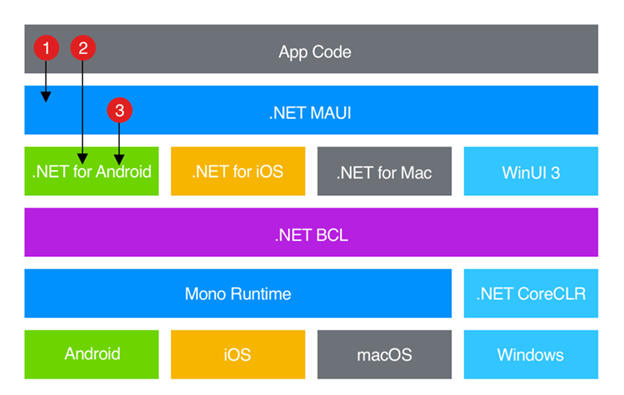
\includegraphics{maui_how_it_works}
    \centering
    \caption[Schematische voorstelling van de bouwstenen van .NET MAUI]{Schematische voorstelling van de bouwstenen van .NET MAUI \autocite{Britch2023}}
    \label{fig:mauiCompilationScheme}
\end{figure}
.NET MAUI voorziet een framework per platform waarmee in C\# geschreven code kan worden gecompileerd voor het gewenste platform. Momenteel heeft .NET MAUI vier platformspecifieke frameworks: .NET voor Android, .NET voor iOS, .NET voor Mac en de Windows UI 3 bibliotheek. Elk van deze frameworks gebruikt de .NET Base Class Library, kortweg BCL, die fungeert als abstractie tussen de geschreven broncode en de verschillende platformen. De BCL vertrouwt op de .NET runtime om de toepassing te compileren. Ook hier zijn verschillende platformspecifieke tools voorzien. Zo is er de Mono runtime voor Android, iOS en macOS, en de .NET CoreCLR voor Windows desktop applicaties \autocite{Britch2023}.

Met BCL kan een toepassing worden gemaakt die op verschillende platforms draait met dezelfde codebasis. Elk platform heeft echter zijn eigen manier om de gebruikersinterface te definiëren, evenals de manier waarop de verschillende elementen met elkaar communiceren en interageren. Dit is waar .NET MAUI u de keuze geeft om verschillende gebruikersinterfaces voor verschillende platformen te creëren of, omgekeerd, één gebruikersinterface voor alle platformen te creëren \autocite{Britch2023}.

\subsection{Een vergelijking tussen .NET MAUI en Xamarin}
Aangezien .NET MAUI de opvolger is van Xamarin.Forms, zijn er veel overeenkomsten, maar ook veel verschillen. In deze sectie worden de twee frameworks met elkaar vergeleken.

Het eerste grote verschil tussen .NET MAUI en Xamarin is de projectstructuur. In Xamarin wordt bij het aanmaken van een project een projectmap per platform aangemaakt, met als gevolg dat platformspecifieke code en resources (zoals fonts, afbeeldingen...) per project moeten worden onderhouden. Met de .NET MAUI wordt een projectmap aangemaakt die meerdere platformmappen bevat. In deze mappen wordt platformspecifieke code opgeslagen \autocite{Koleva2023}.

Het volgende verschil tussen de twee frameworks is de build tooling, .NET MAUI kan de cross-platform .NET CLI (Command Line Interface) gebruiken om projecten te compileren en uit te voeren. Terwijl Xamarin.Forms het .NET framework moet gebruiken om applicaties te bouwen \autocite{Kathiresan2022}.

Een derde belangrijk verschil tussen Xamarin.Forms en de .NET MAUI zijn de platform-specifieke API's. Xamarin biedt een enkele cross-platform API die werkt op Android, iOS en Windows. Met .NET MAUI wordt voor elk platform een API geleverd, waardoor ontwikkelaars kunnen profiteren van de functies van elk platform \autocite{UXDivers}.

Ten slotte kan er met .NET MAUI gekozen worden om de GUI (Graphical User Interface) te bouwen met HTML (HyperText Markup Language) of XAML (Extensible Application Markup Language). Terwijl je met Xamarin.Forms alleen met XAML kan werken \autocite{Kathiresan2022}.

\subsection{Een blik op de toekomst van .NET MAUI}
\begin{figure}[H]
    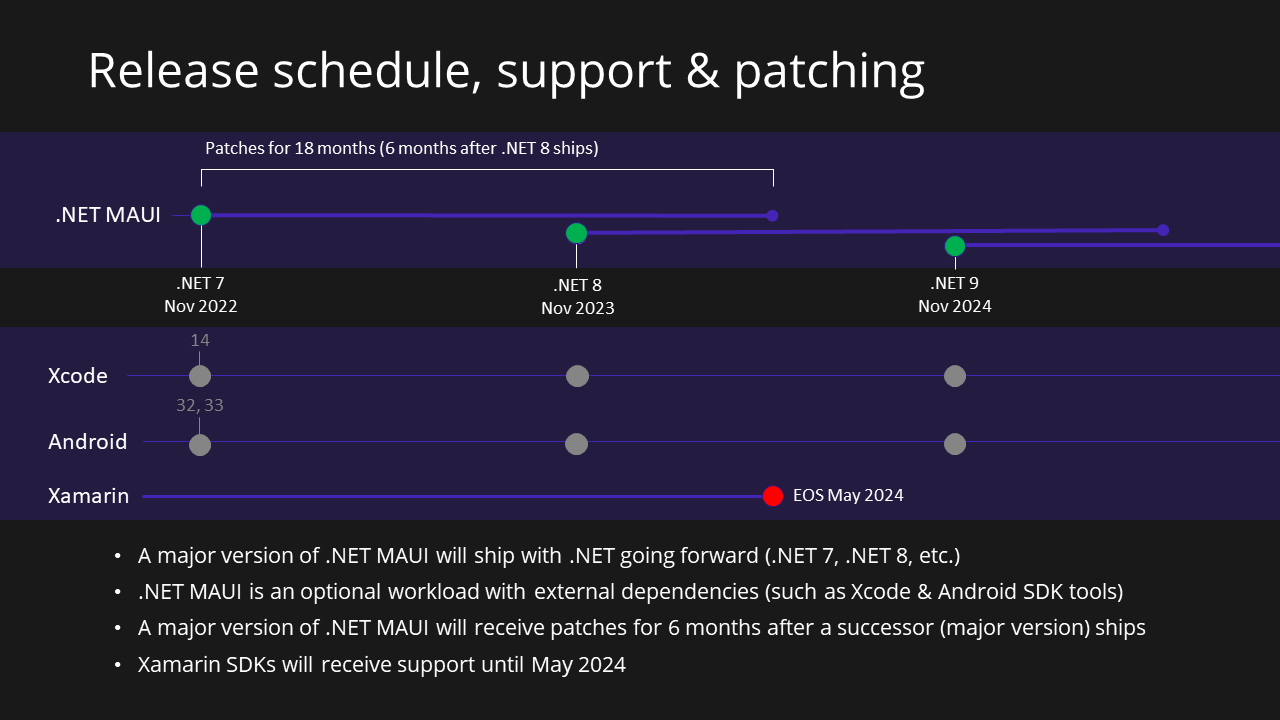
\includegraphics[scale=0.50]{maui_roadmap}
    \centering
    \caption[.NET MAUI release schema]{.NET MAUI release schema \autocite{Ramel2022}}
    \label{fig:mauiRoadMap}
\end{figure}

Elke nieuwe versie van .NET zal vanaf nu ook een major versie van .NET MAUI bevatten. Elk van deze major versies zullen 18 maanden ondersteuning krijgen \autocite{Ramel2022}.

Daarnaast zal de support voor Xamarin.Forms stopgezet worden in mei 2024. Concreet wil dit zeggen dat er geen updates of patches meer zullen uitgebracht worden voor Xamarin.Forms \autocite{Ramel2022}.

\section{Real-time applicaties}
\subsection{Definitie van een real-time applicatie}
Real-time computing verwijst naar computersystemen die zijn ontworpen om gegevensinvoer in real-time te verwerken en erop te reageren, doorgaans binnen milliseconden of microseconden nadat gebeurtenissen zich hebben voorgedaan \autocite{Suse}. 

De reactietijden moeten onmiddellijk lijken en het systeem moet zonder vertraging of onderbreking doorgaan \autocite{Suse}. 

Real-time computing is van cruciaal belang voor toepassingen die onmiddellijke en nauwkeurige gegevensverwerking vereisen, zoals industriële controle, medische toepassingen, luchtvaart, defensie, multimedia, games en financiële handelssystemen \autocite{Suse}. 

Real-time computing vereist gespecialiseerde hardware- en softwarecomponenten, waaronder real-time besturingssystemen, real-time netwerken en synchrone programmeertalen, om het systeem binnen het gewenste tijdsbestek te laten functioneren \autocite{Suse}.

\subsection{HyperText Transfer Protocol}
HTTP is het protocol dat ten grondslag ligt aan het internet. Het protocol wordt gebruikt om gegevensbronnen (zoals HTML, XML, JSON-documenten) op te vragen bij een server \autocite{Cloudflare}.

\begin{figure}[H]
    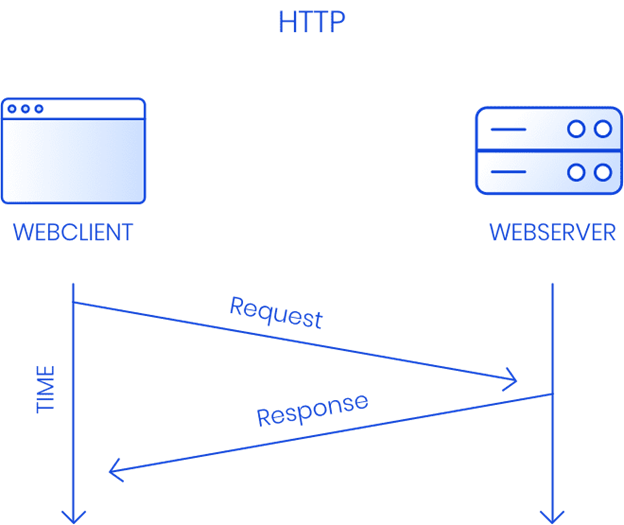
\includegraphics{client_server_scheme}
    \centering
    \caption[Schematische voorstelling van het client-server model]{Schematische voorstelling van het client-server model \autocite{Combell}}
    \label{fig:clientServerScheme}
\end{figure}

HTTP is een client-serverprotocol, wat betekent dat verzoeken om gegevens altijd door de client (ook bekend als de ontvanger) worden geïnitieerd. Het verzoek wordt naar de server gestuurd, die op zijn beurt het gevraagde document samenstelt en terugstuurt als antwoord op het verzoek \autocite{MDN2023}

\begin{figure}[H]
    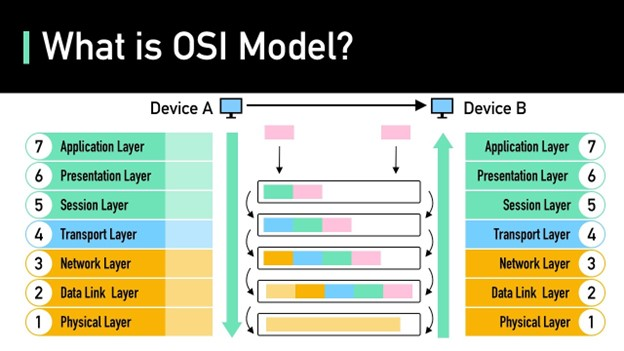
\includegraphics{osi_model}
    \centering
    \caption[Het OSI model]{Het OSI model \autocite{ByteByteGo2022}}
    \label{fig:osiModel}
\end{figure}

Dit protocol is oorspronkelijk voorgesteld door Tim Berners-Lee in 1989 en is gebouwd bovenop de TCP- en IP-protocollen \autocite{MDN2023a}.

Het HTTP-protocol bevindt zich in de zevende laag (ook toepassingslaag genoemd) van het OSI-model \autocite{MDN2023}

De filosofie van HTTP rust op vier pijlers:\\

\begin{itemize}
    \item Uitbreidbaarheid

    De invoering van HTTP-headers in HTTP versie 1 (HTTP/1) \autocite{MDN2023a} maakt het mogelijk extra informatie toe te voegen aan verzoeken en antwoorden, zolang client en server deze overeenkomst aanvaarden \autocite{Paessler}.
    
    \item Staatloos
    
    Staatloos betekent dat tijdens en na het verzenden en ontvangen van een verzoek en antwoord geen informatie door de server wordt bijgehouden. Met andere woorden, elk verzoek dat de server ontvangt wordt onafhankelijk gezien en uitgevoerd. Een stateless protocol is ontworpen met het oog op schaalbaarheid. Afhankelijk van de werklast kunnen dus meerdere servers worden opgezet met dezelfde informatie, en elke server in de configuratie kan het verzoek ontvangen en verwerken \autocite{Paessler}.
    
    Om een toestand bij te houden kunnen HTTP-cookies worden gebruikt. Dit is mogelijk dankzij de bovengenoemde uitbreidbaarheid en maakt het mogelijk bepaalde informatie (zoals authenticatietokens) te delen tussen meerdere verzoeken \autocite{MDN2023}.
    
    \item Verbindingsloos
    
    Het HTTP-protocol wordt om twee redenen als verbindingsloos beschouwd. Omdat verbindingen worden gemaakt door de transportlaag (laag 4 van het OSI-model), valt het niet onder de verantwoordelijkheid van een applicatie laag (laag 7 van het OSI-model) applicatie \autocite{MDN2023}.
    
    Bovendien worden voor elk verzoek verbindingen gelegd tussen de client en de server. Zodra het verzoek is verwerkt, sluit de server de verbinding \autocite{Paessler}.
    
    \item Media onafhankelijk
    
    Zolang de client en de server weten hoe zij bepaalde door het MIME-type (Multipurpose Internet Mail Extensions) gespecificeerde gegevens moeten verwerken, kunnen de gegevens via het HTTP-protocol worden getransporteerd \autocite{Paessler}.
\end{itemize}

\subsubsection{De evolutie van het HTTP-protocol}
\emph{HTTP/0.9}

Aanvankelijk had het HTTP-protocol geen versienummer (aangegeven door het cijfer achter het teken /). Om de verschillende versies van elkaar te scheiden, kreeg de allereerste implementatie van het HTTP-protocol echter versienummer 0.9 \autocite{MDN2023a}.

Met verzoeken die bestaan uit een enkele regel bestaande uit het type verzoek en de naam van de gegevensbron, is deze versie van HTTP vrij primitief. Ook kan met deze versie alleen een GET-verzoek worden gedaan. Bijgevolg kunnen alleen gegevens worden gelezen \autocite{Grigorik}


\emph{HTTP/1.0}
HTTP-versie 1.0 werd uitgebracht in 1990, vijf jaar nadat versie 0.9 was geïntroduceerd, en voegde nieuwe functies toe om eerdere tekortkomingen te verhelpen:

\begin{itemize}
    \item HTTP-header
    
    Zoals hierboven vermeld, bestond een verzoek van versie 0.9 alleen uit de methode en de naam van de gegevensbron die werd opgevraagd \autocite{FulberGarcia2022}.
    Door de toevoeging van de HTTP-header kunnen nu metadata worden opgenomen in verzoeken en antwoorden, wat deze versie van het protocol flexibel en uitbreidbaar maakt \autocite{MDN2023a}.
    
    \item Versiebeheer
    
    Elk HTTP-verzoek bevat nu de gebruikte HTTP-versie \autocite{MDN2023a}.
    
    \item Statuscode
    
    Aan elk antwoord wordt een statuscode toegevoegd. Dit is een manier voor de client om bij elk antwoord te controleren of het verzoek al dan niet correct is verwerkt \autocite{FulberGarcia2022}.
    
    \item Content-type
    
    Zoals hierboven vermeld, kunnen met de HTTP-header extra metadata aan een verzoek worden toegevoegd. Voor HTTP/1.0 is nu een inhoudstype in de header opgenomen, waardoor ook andere documenten dan HTML kunnen worden verzonden \autocite{FulberGarcia2022}.
    
    \item Extra methoden
    
    HTTP/1.0 heeft ten slotte twee nieuwe methoden toegevoegd, POST en HEAD. Dit zorgt ervoor dat gegevens nu zowel geschreven als gelezen kunnen worden \autocite{FulberGarcia2022}.
\end{itemize}


\emph{HTTP/1.1}
\begin{figure}
    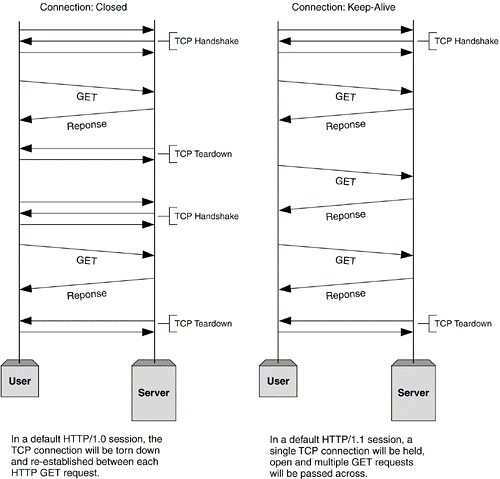
\includegraphics{http_1.0_vs_http_1.1_connections}
    \centering
    \caption[Schematische voorstelling van het verschil tussen niet-herbruikbare en herbruikbare connecties van respectievelijk HTTP/1.0 en HTTP/1.1]{Schematische voorstelling van het verschil tussen niet-herbruikbare en herbruikbare connecties van respectievelijk HTTP/1.0 en HTTP/1.1 \autocite{Hesham2019}}
    \label{fig:httpConnectionScheme}
\end{figure}

HTTP/1.1 werd een jaar na de release van HTTP/1.0 geïmplementeerd. Dit was slechts bedoeld als een verbetering van de 1.0-versie:

\begin{itemize}
    \item Host header
    
    Met HTTP/1.1 moet de client het host veld toevoegen aan de header van elke aanvraag. Vóór deze versie was dit niet verplicht. Dankzij dit veld kunnen verzoeken via een proxyserver naar de juiste server worden geleid. In de praktijk betekent dit dat als er verschillende domeinen naar dezelfde locatie verwijzen, er toch een onderscheid kan worden gemaakt om ervoor te zorgen dat het verzoek niet naar de verkeerde server gaat \autocite{FulberGarcia2022}.
    
    \item Persistente verbinding
    
    Zoals hierboven vermeld, moest de client in HTTP-versie 1.0 een verbinding maken voor elk verzoek dat hij wilde verzenden. In versie 1.1 kan de verbinding open worden gehouden totdat de client aangeeft dat hij de verbinding wil sluiten \autocite{MDN2023a}.
    
    \item Continue-status
    
    Vóór de invoering van de continue status konden sommige verzoeken niet door de server worden verwerkt. Als dit het geval was, werd het verzoek gewoon onbeantwoord afgewezen. Vanaf versie 1.1 kan een client eerst de HTTP-headers van het verzoek aan de server doorgeven. Als de server antwoordt met de status continue (statuscode 100), weet de client dat hij het hele verzoek kan doorsturen en een antwoord van de server kan verwachten \autocite{FulberGarcia2022}.
    
    \item Aanvullende methoden
    
    Versie 1.1 introduceert ook een aantal nieuwe methoden. Deze omvatten PUT, PATCH, DELETE, CONNECT, TRACE en OPTIONS \autocite{FulberGarcia2022}.
\end{itemize}


\emph{HTTP/2.0}

HTTP/2.0 is uitgebracht in 2015, 18 jaar na 1.1. Het is echter nog niet op grote schaal ingevoerd. Het gebruik van HTTP/2.0 is dan ook een bewuste keuze van de ontwikkelaars \autocite{Ab}.
HTTP/2.0 brengt een aantal nieuwe functies die nieuwe mogelijkheden bieden, namelijk:

\begin{itemize}
    \item Multiplexing
    
    In versie 1.1 van het HTTP-protocol werden verzoeken om gegevens sequentieel verwerkt. Dat wil zeggen, het eerste HTML-document werd opgevraagd en geladen, dan het tweede document, enzoverder tot alles geladen was. Dit kon echter tot problemen leiden als een bepaalde bron niet kon worden geladen omdat de rest van de bron werd opgehouden. Met HTTP/2.0 kan één enkele TCP-verbinding worden gebruikt om meerdere verzoeken tegelijk te doen. Dit zorgt ervoor dat wanneer het bovengenoemde probleem zich voordoet, de resterende gegevens al kunnen worden geladen \autocite{Cloudflare}.
    
    \item Server push
    
    Vóór de invoering van HTTP/2.0 kon de server alleen gegevens naar de client pushen nadat deze een verzoek had verzonden. In versie 2.0 is echter server push geïmplementeerd. Hierdoor kan de server gegevens naar de client sturen nog voordat de client een verzoek naar hem heeft gestuurd. Dit lost prestatieproblemen met lange polling op \autocite{Grigorik2016}.
    
    \item Compressie van headers
    
    De toevoeging van HTTP-headers aan een verzoek vergroot de omvang van het verzoek. Dit kan leiden tot het langzamer laden van gegevens en het langzamer verwerken van gegevens door de client. Deze verzoeken kunnen kleiner worden gemaakt en sneller worden verwerkt door de headers te comprimeren. HTTP/1.1 deed dit al, maar versie 2.0 heeft een veel verfijnder compressie-algoritme, het HPACK-algoritme. Dit algoritme verwijdert alle overbodige informatie, waardoor verzoeken kleiner worden \autocite{Cloudflare}.
\end{itemize}

\subsection {WebSocket protocol}

Het WebSocket protocol is een relatief nieuw protocol. Het protocol werd voor het eerst beschreven in 2008 door Micahel Carter en Ian Hickson en kreeg algemene ondersteuning rond 2010 \autocite{Ably2020}.

In december 2011 publiceerde het IETF (Internet Engineering Task Force) de whitepaper die het WebSocket protocol beschreef onder de titel ``RFC 6455 - The WebSocket Protocol'' \autocite{Fette2011}.

Volgens de paper van \textcite{Fette2011} is het WebSocket protocol ontwikkeld om real-time applicaties mogelijk te maken zonder het zogenaamde ``HTTP long polling'' te misbruiken.

Bij HTTP long polling stuurt de client een aanvraag uit naar de server. In plaats van direct te antwoorden en daarna de connectie te sluiten, wacht de server met antwoorden totdat er nieuwe data beschikbaar is. Na het uitsturen van het antwoord, krijgt de server meteen een nieuwe aanvraag van de client \autocite{Singh}. 

Het WebSocket protocol is full-duplex en laat bidirectionele communicatie toe. Concreet betekent dit dat in plaats van een aanvraag te sturen die enkel beantwoord wordt wanneer er nieuwe data is, het nu mogelijk is om data door te sturen naar de client zonder dat deze een aanvraag verstuurd heeft. Dit zorgt voor een betere performantie ten opzichte van het HTTP long polling \autocite{Fette2011}

\begin{figure}[H]
    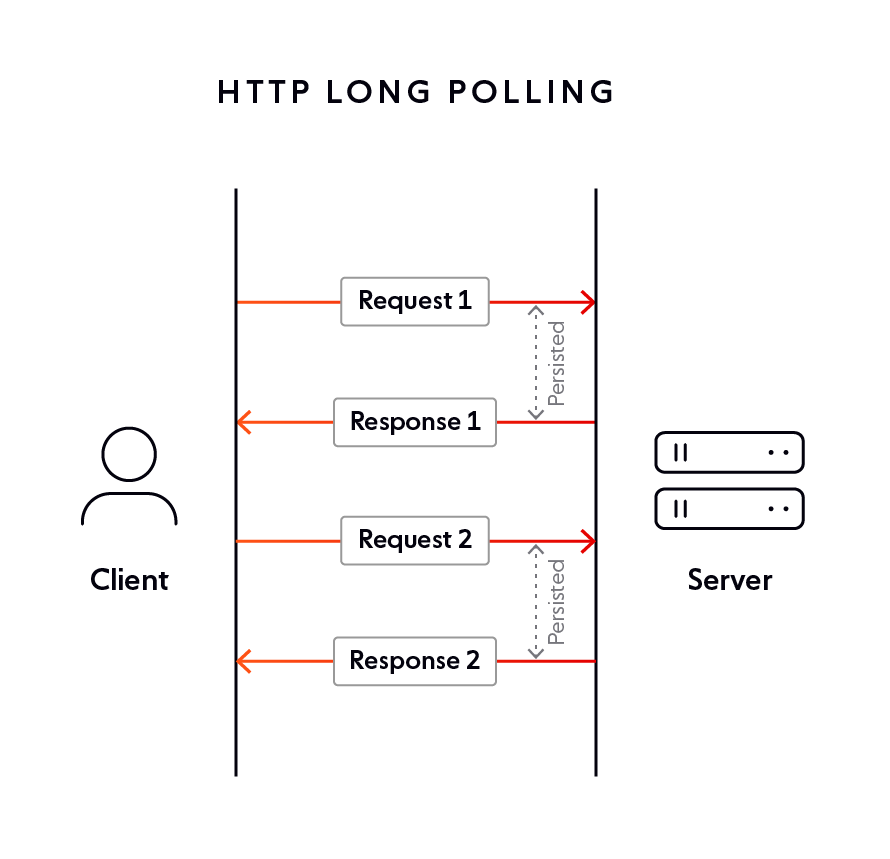
\includegraphics{http_long_polling}
    \centering
    \caption[Schematische voorstelling van HTTP long polling]{Schematische voorstelling van HTTP long polling \autocite{Ably2020}}
    \label{fig:httpLongPolling}
\end{figure}

\subsection{Real-time programmeren binnen het .NET ecosysteem}
De ASP.NET SignalR bibliotheek is beschikbaar voor real-time applicatieontwikkeling binnen het .NET ecosysteem. Deze bibliotheek maakt het mogelijk een tweerichtingscommunicatie op te zetten tussen een client en een server. De client kan met name bepaalde functies op de server aanroepen, maar de server kan ook functies opvragen bij de client \autocite{BradyGaster2020}.

In het traditionele client-server model kan alleen de client functies op de server aanroepen. Dit betekent dat als de gegevens zo actueel mogelijk moeten zijn, er extra logica moet worden geïmplementeerd om de server na een bepaald aantal seconden te polsen naar de (mogelijk) gewijzigde gegevens (deze implementatie wordt ook wel "long polling" genoemd). Dit kan leiden tot slecht presterende toepassingen \autocite{BradyGaster2020}.

Dankzij het gebruik van SignalR is het nu ook mogelijk dat de server functies gaat aanroepen op de client. Dit zorgt ervoor dat het hierboven getoonde voorbeeld op een veel performantere manier kan worden geïmplementeerd. Wanneer gegevens op de server worden gewijzigd, kan de server alle luisterende clients opdragen de nieuwe gegevens op te halen. Dit zorgt ervoor dat gegevens alleen worden opgevraagd wanneer de gegevens veranderen, in plaats van telkens na een bepaalde periode \autocite{BradyGaster2020}.
%%=============================================================================
%% Methodologie
%%=============================================================================

\chapter{\IfLanguageName{dutch}{Methodologie}{Methodology}}%
\label{ch:methodologie}

%% TODO: Hoe ben je te werk gegaan? Verdeel je onderzoek in grote fasen, en
%% licht in elke fase toe welke stappen je gevolgd hebt. Verantwoord waarom je
%% op deze manier te werk gegaan bent. Je moet kunnen aantonen dat je de best
%% mogelijke manier toegepast hebt om een antwoord te vinden op de
%% onderzoeksvraag.

\subsubsection{Inleiding}
Tijdens het opstellen van deze bachelorproef hebben twee grote activiteiten plaatsgevonden, namelijk een literaire studie en het opstellen van een proof-of-concept. 

\begin{itemize}
    \item Literaire studie
    
    De literaire studie heeft als doel een gepast referrentiekader te geven voor elke lezer van deze proef.
    
    \item proof-of-concept
    
    Het doel van de proof-of-concept is om een conclusie te kunnen vormen op de onderzoeksvraag.
\end{itemize}

In dit hoofdstuk wordt de wijze waarop deze twee activiteiten zijn uitgevoerd verduidelijkt.

\section{Theoretisch onderzoek}
\subsection{Fase 1}
Het doel van de eerste fase van het literaire onderzoek was het bepalen van de in dit onderzoek op te nemen onderwerpen. 

Hierbij was het van groot belang dat de lezer van deze proef de juiste contextualisering krijgt. Daarnaast was het ook belangrijk om enkel de juiste onderwerpen te vermelden.

\subsection{Fase 2}
De doelstelling van deze fase was onderzoek te voeren naar de geschiedenis van de COBOL programmeertaal en hoeveel er nog gebruik gemaakt wordt van deze programmeertaal in de huidige technologische markt.

\subsection{Fase 3}
Tijdens deze fase werd er onderzocht wat native en cross-platform development is en welke voor- en nadelen deze twee manieren van werken met zich meebrengen.

\subsection{Fase 4}
Tijdens fase 4 werd er onderzoek gedaan naar wat .NET MAUI is, hoe het werkt, hoe het zich verhoudt ten op zichte van zijn voorganger Xamarin.Forms en hoe de toekomst eruitziet voor het nieuwste framework van Microsoft.

\subsection{Fase 5}
Bij het uitvoeren van het onderzoek voor deze fase werd er getracht om eerst de term ``real-time applicatie'' te definiëren, waarna werd onderzocht wat het HTTP protocol is en hoe dit geëvolueerd is ten opzichte van de eerste versie. Daarna werd onderzocht wat het WebSocket protocol is en waarom dit ontwikkeld is. Tot slot werd de SignalR bibliotheek van Microsoft bestudeerd in verband met het real-time programmeren binnen .NET.

\section{Proof-of-concept}
Na het uitvoeren van het literaire onderzoek werd de proof-of-concept opgezet. Ook dit werd gefaseerd uitgevoerd.

\subsection{Fase 1}
Tijdens deze fase werd eerst en vooral een opsomming gemaakt van welke applicaties er nodig zijn om de proof-of-concept volledig op te kunnen zetten en welke apparatuur en software hiervoor noodzakelijk zijn.

Daarna werd de systeemarchitectuur opgesteld. Hiervoor werd een schema gemaakt van welke apparaten met elkaar in verbinding zouden staan en welke applicaties op welke apparaten zouden draaien.

Tot slot werd het domeinklassediagram ontworpen. Dit diagram toont welke klassen er nodig zijn, welke associaties, eigenschappen en methoden deze hebben.

\subsection{Fase 2}
In fase 2 werd het domeinklassediagram omgezet in concrete klassen en werden enkele van deze klassen getest om te controleren of de geïmplementeerde logica het verwachte resultaat oplevert.

\subsection{Fase 3}
Deze fase had als doelstelling het volledig implementeren van de applicaties die in de winkel moeten draaien, namelijk: de management API, de operations API en de operations client. 

De management API moet een winkel-, printer- en staffelobject kunnen configureren en persisteren in de databank.

De operations API moet een verkoopobject kunnen aanmaken, het totaal te betalen bedrag kunnen berekenen, de digitale signalen, uitgestuurd door het python script, ontvangen en de tellerstanden van de printers op de GUI updaten.

De operations client dient als grafische interface voor de winkelverantwoordelijke. Deze moet toelaten om de huidige tellerstand van de printers te bekijken, het commando uitsturen om het totaal te betalen bedrag te berekenen, een verkoop te registreren en bij het afsluiten van het systeem moet er een aanvraag verstuurd worden naar de reporting API.

\subsection{Fase 4}
Tijdens deze fase werd het python script geschreven. Dit script moest dienen om te luisteren naar de seriële verbinding tussen de Arduino en Raspberry Pi en indien er boodschappen staan te wachten, deze berichten decoderen. Eens deze gedecodeerd zijn wordt er een PATCH-aanvraag verstuurd naar de operations API met als parameter het interfacenummer waarop het analoge signaal geregistreerd werd.

\subsection{Fase 5}
Bij het uitvoeren van fase 5 was het de bedoeling om de dagrapporten applicaties volledig te implementeren. Concreet betekent dit dat de reporting API werd opgesteld. Deze heeft als doel om een nieuw dagrapport voor een winkel te genereren, te persisteren in de databank en een push-notificatie te versturen naar de reporting client.

Daarnaast werd ook de reporting client ontwikkeld. Dit is een mobiele applicatie die dient als dashboard waarop de zaakvoerder bepaalde datavisualisaties kan bekijken omtrent het aantal verkopen in de copycentra. Deze moet de push-notificatie verzonden door de reporting API ontvangen en een melding geven aan de zaakvoerder dat er een nieuw dagrapport beschikbaar is.

\subsection{Fase 6}
Na het opstellen van de proof-of-concept is er ook nog een extra tool ontwikkeld om metingen uit te kunnen voeren. Deze verstuurt een digitaal signaal analoog aan het signaal dat verstuurd wordt door de Arduino. Het tijdstip waarop het signaal verstuurd en beantwoord wordt, wordt geregistreerd. Daarna wordt het tijdsverschil tussen deze twee punten berekend en weggeschreven naar een CSV-file (Comma Seperated Value). Met andere woorden, deze tool simuleert het python listener script en meet de responsetijd van de .NET MAUI applicatie.

% Voeg hier je eigen hoofdstukken toe die de ``corpus'' van je bachelorproef
% vormen. De structuur en titels hangen af van je eigen onderzoek. Je kan bv.
% elke fase in je onderzoek in een apart hoofdstuk bespreken.

%\input{...}
%\input{...}
%...

%%=============================================================================
%% Conclusie
%%=============================================================================

\chapter{Conclusie}%
\label{ch:conclusie}

% onderzoeksvra(a)g(en). Wat was jouw bijdrage aan het onderzoeksdomein en
% hoe biedt dit meerwaarde aan het vakgebied/doelgroep? 
% Reflecteer kritisch over het resultaat. In Engelse teksten wordt deze sectie
% ``Discussion'' genoemd. Had je deze uitkomst verwacht? Zijn er zaken die nog
% niet duidelijk zijn?
% Heeft het onderzoek geleid tot nieuwe vragen die uitnodigen tot verder 
%onderzoek?
\subsubsection{Inleiding}
In dit hoofdstuk zal er getracht worden een conclusie te formuleren op de hoofdonderzoeksvraag en diens subvragen.

\section{Subonderzoeksvraag 1}
Na het opstellen van de proof-of-concept werden er metingen uitgevoerd op zowel het bestaande systeem als de proof-of-concept. Dit met als doel een conclusie op de tweede subonderzoeksvraag, namelijk: ``Wat is de gemiddelde reactiesnelheid van de .NET MAUI applicatie en hoe verhoudt deze zich ten opzichte van de gemiddelde reactiesnelheid van het huidige systeem?''

De hypothese voor deze vraag luidt als volgt: ``de gemiddelde reactietijd van de POC is kleiner dan de gemiddelde reactietijd van de huidige applicatie''

Om de hypothese te kunnen aannemen of verwerpen werden enkele statistische toetsen uitgevoerd:

\begin{enumerate}
    \item Het gemiddelde van de twee datasets werd berekend
    
    \begin{itemize}
        \item Voor het huidige systeem is het gemiddelde gelijk aan 1867,076
        
        \item Voor de proof-of-concept is het gemiddelde gelijk aan 523,931
    \end{itemize}

    Hieruit kan al geconcludeerd worden dat de gemiddelde reactiesnelheid van de proof-of-concept veel lager is dan de reactiesnelheid van het huidig systeem.

    \item Een twee-sample T-test werd uitgevoerd. Deze test zou een definitief antwoord moeten geven over de geldigheid van de hypothese. Voor deze test werd een significantieniveau van 0,05 gebruikt. Daarnaast werden ook twee hypotheses opgesteld, namelijk:
    
    \begin{itemize}
        \item H0: de gemiddelde reactietijd van de POC is groter of gelijk aan de gemiddelde reactietijd van de huidige applicatie
        
        \item H1: de gemiddelde reactietijd van de POC is kleiner dan de gemiddelde reactietijd van de huidige applicatie
    \end{itemize}

    Na het uitvoeren van deze test werd een p-waarde, ook wel de overschrijdingskans genoemd, vastgesteld die ongeveer gelijk was aan nul. Aangezien de p-waarde kleiner is dan het bovengenoemde significantieniveau, mag de nulhypothese verworpen worden.
\end{enumerate}

Kortom beide statistische proeven tonen aan dat de initiële hypothese klopt. Daarnaast kan er dankzij deze twee proeven ook een antwoord op de onderzoeksvraag geformuleerd worden, namelijk: de gemiddelde reactiesnelheid van de .NET MAUI-applicatie is gelijk aan 523,931 en is in verhouding tot het huidig systeem 3,56 keer zo snel op vlak van reactietijd.

\begin{figure}[H]
    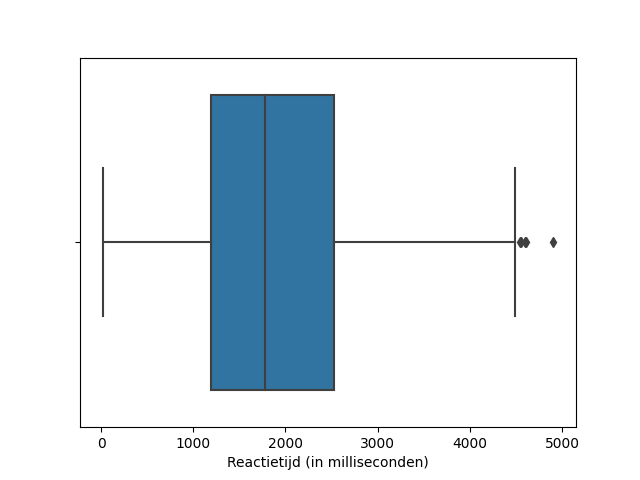
\includegraphics{Current_Plot_Boxplot}
    \centering
    \caption{Boxplot van de reactietijden in het huidige syteem}
    \label{fig:httpLongPolling}
\end{figure}

\begin{figure}[H]
    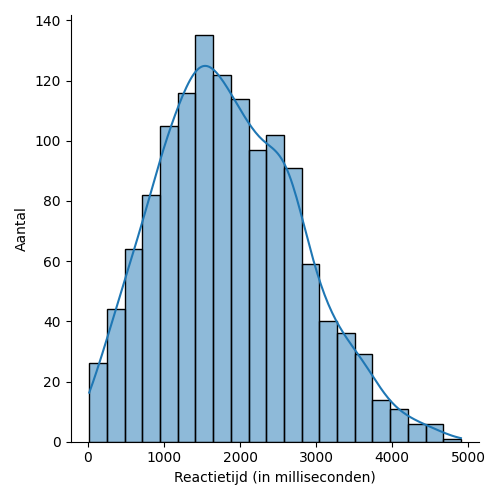
\includegraphics{Current_Plot_Histogram}
    \centering
    \caption{Histogram van de reactietijden in het huidige syteem}
    \label{fig:httpLongPolling}
\end{figure}

\begin{figure}[H]
    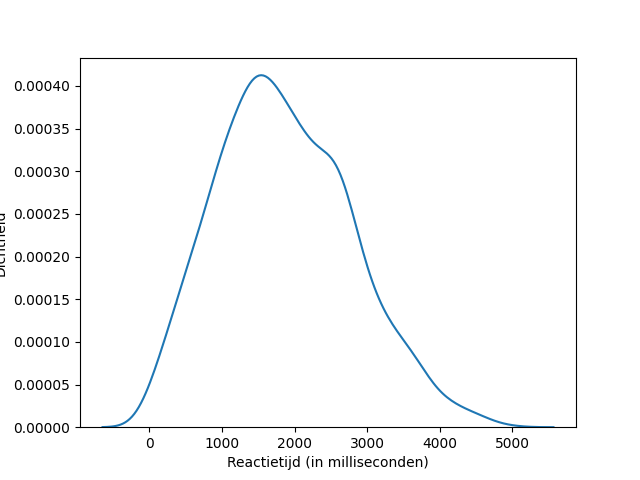
\includegraphics{Current_Plot_Density}
    \centering
    \caption{Densiteitsgrafiek van de reactietijden in het huidige sysyteem}
    \label{fig:httpLongPolling}
\end{figure}

\begin{figure}[H]
    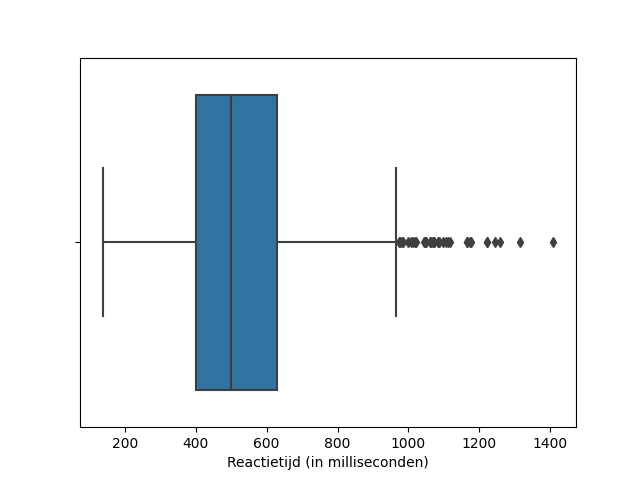
\includegraphics{POC_Plot_Boxplot}
    \centering
    \caption{Boxplot van de reactietijden in de proof-of-concept}
    \label{fig:httpLongPolling}
\end{figure}

\begin{figure}[H]
    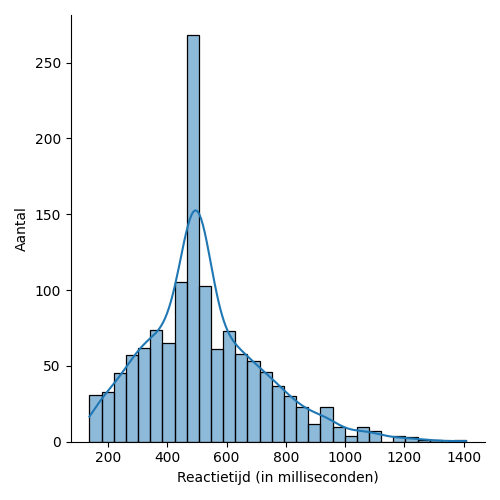
\includegraphics{POC_Plot_Histogram}
    \centering
    \caption{Histogram van de reactietijden in de proof-of-concept}
    \label{fig:httpLongPolling}
\end{figure}

\begin{figure}[H]
    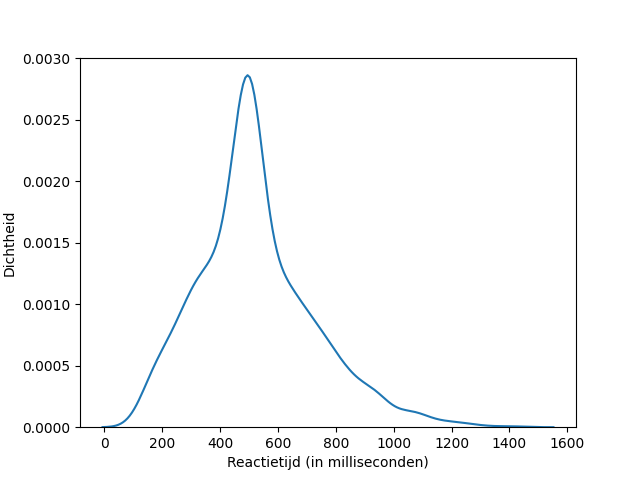
\includegraphics{POC_Plot_Density}
    \centering
    \caption{Densiteitsgrafiek van de reactietijden in de proof-of-concept}
    \label{fig:httpLongPolling}
\end{figure}

\section{Subonderzoeksvraag 2}
Het tweede luik van de onderzoeksvraag luidt als volgt: ``Laat .NET MAUI het toe om push-notificatie te versturen?''

.NET MAUI levert geen algemene bibliotheek aan om push-notificaties te implementeren in de mobiele applicaties. Om dit te kunnen verwezenlijken, moeten we voor ieder platform een verschillend project opzetten die enkel de applicatie voor dat platform kan gaan bouwen. Daarnaast is er ook nood aan het gebruik van een bibliotheek uitgegeven door een derde partij. In dit geval gaat het om de Plugin.Firebase biblitoheek gemaakt en onderhouden door Tobias Buchholz. Dit zorgt ervoor dat de applicatie moet steunen op Firebase, wat een verzameling is van backend cloud computing services aangeboden door Google.

Dit alles zorgt ervoor dat er geconludeerd kan worden dat .NET MAUI het wel toelaat om push-notificaties te versturen, maar dat dit niet eenmalig geïmplementeerd kan worden voor de drie platformen samen. Dit zorgt er dan ook voor dat enkele van de voordelen van een cross-platform framework wegvallen.

\section{Algemene conclusie}
Door de conclussies geformuleerd voor de twee subonderzoeksvragen kan nu ook een algemeen besluit gevormd worden. Zoals in de inleiding wordt vermeld is het onderzoek een partiëel succes wanneer een positief besluit gevormd kan worden voor de eerste subonderzoeksvraag. Deze proef is een compleet succes wanneer de tweede subonderzoeksvraag een positief resultaat verkrijgt.

Dit onderzoek is alvast een partiëel succes aangezien het antwoord op de vraag: ``Wat is de gemiddelde reactiesnelheid van de .NET MAUI applicatie en hoe verhoudt deze zich ten opzichte van de gemiddelde reactiesnelheid van het huidige systeem?'' als volgt luidt: ``De gemiddelde reactiesnelheid van .NET MAUI is gelijk aan 523,931 en is in verhouding tot de gemiddelde reactiesnelheid van het huidige systeem 3,56 keer zo snel''.

Over het complete succes van de proef kan gedebateerd worden aangezien het mogelijk is om push-notificaties te versturen. Echter is dit momenteel enkel mogelijk indien er voor de verschillende platformen een aparte codebase wordt gebouwd (wat indruist tegen de visie van .NET MAUI) en er geen standaard bibliotheken aangeleverd worden door Microsoft. In deze proef wordt dit dan ook niet aanzien als een succes.

Dit alles zorgt er voor dat de algemene conclusie van deze proef als volgt luidt: .NET MAUI is voldoende matuur om een POS-systeem geschreven in COBOL te vervangen. Echter wanneer nood is aan het gebruik van niche features, zoals bijvoorbeeld het gebruik van push-notificaties, heeft .NET MAUI nog wat zaken die (beter) geïmplementeerd moeten worden.

%---------- Bijlagen -----------------------------------------------------------

\appendix

\chapter{Onderzoeksvoorstel}

Het onderwerp van deze bachelorproef is gebaseerd op een onderzoeksvoorstel dat vooraf werd beoordeeld door de promotor. Dat voorstel is opgenomen in deze bijlage.

\section*{Samenvatting}

Native applicatie development is een tijdrovend en duur proces waarbij een applicatie ontwikkeld wordt voor verschillende platformen, zoals iOS en Android. Hier kan cross-platform development een goede oplossing bieden. Cross-platform laat toe om met één codebase in één en dezelfde programmeertaal een applicatie te ontwikkelen die op de meeste gebruikte platformen kan draaien. In deze bachelorproef zal er worden nagegaan of .NET MAUI al voldoende ontwikkeld is om een real-time kassa-applicatie, geschreven in COBOL, te vervangen met een productiewaardige cross-platform applicatie ontwikkeld in .NET.
In de eerste fase van het onderzoek zal er nagegaan worden of het analoge signaal van een printer opgevangen en omgevormd kan worden met een Raspberry Pi.
In de tweede fase zal er een real-time .NET MAUI-applicatie ontwikkeld worden die steeds kan worden geüpdate wanneer er een signaal van een printer binnenkomt.
Tenslotte zal de .NET MAUI-applicatie gecompileerd worden naar een mobiel platform. Hier zal nagegaan worden of dit zonder enige probleem kan.
Er wordt verwacht dat de .NET MAUI-applicatie sneller zal reageren dan de huidige COBOL-applicatie. Daarnaast wordt er ook aangenomen dat de user experience al zodanig ontwikkeld is dat er slechts kleine problemen zouden voorkomen bij het compileren naar een mobiel platform.
De beoogde doelgroep voor dit onderzoek is elke ontwikkelaar die de overweging maakt om .NET MAUI te gebruiken om een cross-platform applicatie te ontwikkelen.

% Verwijzing naar het bestand met de inhoud van het onderzoeksvoorstel
%---------- Inleiding ---------------------------------------------------------

\section{Introductie}%
\label{sec:introductie}

Een bedrijf (Goossens NV) heeft enkele copycentra, waar ze momenteel nog steeds werken met een kassasysteem dat geschreven is in COBOL. Op het einde van de dag wanneer de winkel sluit, moet steeds een dagrapport worden gemaakt en deze worden dan op een floppydisk geplaatst. Aan het begin van afgelopen zomer stoot het bedrijf op het probleem dat er geen floppydisks meer geproduceerd worden. Dit heeft als gevolg dat de dagrapporten niet meer bewaard kunnen worden. In dit onderzoek zal worden nagegaan of .NET MAUI, een cross-platform programmeertaal, al voldoende ontwikkeld is om een nieuw real-time kassasysteem op te zetten.

%---------- Stand van zaken ---------------------------------------------------

\section{State-of-the-art}%
\label{sec:state-of-the-art}

\subsection{Cross-platform development}
Cross-platform development, ook wel multi-platform development genoemd, is een manier van ontwikkelen dat toelaat om met één programmeertaal en bijgevolg één codebase een applicatie te ontwikkelen die op verschillende platformen kan draaien \autocite{KotlinFoundation2022}. 

\subsubsection{Native development VS cross-platform development}
De term “native development” geeft aan dat een applicatie uitsluitend ontwikkeld wordt voor één bepaald platform, bijvoorbeeld iOS. De applicatie wordt geprogrammeerd met de door dat platform voorziene programmeertaal en hulpmiddelen \autocite{Marchuk}.

Om native Android-applicaties te schrijven, moet de developer gebruik maken van Java of Kotlin. De talen, die dan weer native ondersteund worden door het iOS platform, zijn Objective-C en Swift \autocite{Schmitt2022}.

\subsubsection{.NET MAUI}
.NET MAUI is de uitgebreide evolutie van Xamarin.Forms om niet alleen mobiele applicaties te ontwikkelen, maar ook desktopapplicaties. .NET MAUI verenigt Android, iOS, macOS en Windows API’s in een enkele API  die het toelaat om met één codebase applicaties te ontwikkelen voor de verschillende platformen \autocite{Britch2022}.

\subsection{Real-time applicaties}
De term real-time applicatie wordt door \textcite{Lutkevich2022} als volgt gedefinieerd:
“Real-time-toepassingen zijn toepassingen die binnen een onmiddellijk tijdskader werken; zij detecteren, analyseren en handelen op streaming gegevens terwijl die zich voordoen. Dit in tegenstelling tot een database-gerichte toepassing waarbij informatie wordt opgenomen en opgeslagen in een database (in de cloud of op locatie) voor toekomstige analyse.”

Om de werking van real-time applicaties te kunnen verduidelijken, moet het websocket protocol uitgelegd worden.

\subsubsection{HyperText Transfer Protocol}
HyperText Transfer Protocol, ook wel gekend als HTTP, is het standaard protocol dat webbrowsers gebruiken om informatie op te vragen bij de server. HTTP werkt volgens het client-server principe. Dit houdt in dat de client, in de meeste gevallen de webbrowser, steeds een dataverzoek stuurt naar de server. Deze zal op zijn beurt dan de gewenste data verzamelen en terugsturen als een document van een bepaald type. Dit kan bijvoorbeeld gaan over HTML-documenten voor webpagina’s of JSON-documenten om data te transfereren \autocite{MDN2022}.

Zoals hierboven beschreven is HTTP unidirectioneel. Dit wil zeggen dat de data-aanvragen enkel en alleen kunnen worden opgestart door een client en kunnen alleen beantwoord worden door de server. Na versturen van het antwoord, wordt de verbinding verbroken \autocite{MDN2022}.

\subsubsection{WebSocket}
WebSocket is een bidirectioneel protocol die dezelfde noden vervult als HTTP, maar in tegenstelling tot HTTP is WebSocket een stateful protocol. Hiermee wordt bedoeld dat de verbinding tussen de client en de server in stand wordt gehouden ook al is de data aanvraag verwerkt. De enige manier om de verbinding te verbreken is wanneer één van de twee partijen besluit om de verbinding stop te zetten. Een groot verschil met HTTP is ook dat de communicatie bij WebSocket bidirectioneel is, wat wil zeggen dat de client de server kan aanspreken, maar ook dat de server de client kan aanspreken \autocite{GeeksforGeeks2022}.

%---------- Methodologie ------------------------------------------------------
\section{Methodologie}%
\label{sec:methodologie}
Het huidige kassasysteem werkt als volgt: een klant komt binnen in één van de copy centra en krijgt een printer aangewezen door de verko(o)p(st)er die op dat moment in de winkel staat. Eens de klant het printproces gestart heeft, wordt er per geprinte pagina een klik doorgestuurd naar een elektronisch bord. Dit bord weet op welke interface de klik binnengekomen is, welke printer het signaal verstuurd heeft en vertaalt dit dan naar een digitaal signaal dat verstuurd wordt naar het kassasysteem. Eens het signaal is aangekomen, wordt de GUI geüpdatet zodat op het einde van het printproces de verkoopster exact weet hoeveel pagina’s er geprint zijn en hoeveel het te betalen totaal is.

Hieruit kunnen volgende onderzoeksvragen naar voor geschoven worden:
\begin{enumerate}
    \item Is .NET MAUI voldoende ontwikkeld om het bestaande kassasysteem te vervangen?
    \item  Is het mogelijk om de desktop applicatie te vertalen naar een mobiel platform?
    \item Is de ontwikkelde .NET MAUI-applicatie sneller in het verwerken van de printerklik dan de huidige applicatie. 
\end{enumerate}
Om na te gaan of .NET MAUI al voldoende ontwikkeld is voor deze toepassing zal er een proof-of-concept opgezet worden. In de eerste fase zal er uitgezocht worden of het analoge signaal, de zogenaamde klik, kan worden opgevangen door een Raspberry Pi en kan worden vertaald naar een digitaal signaal.

In het tweede luik van het onderzoek zal er een .NET MAUI-applicatie worden ontwikkeld die het huidige COBOL-kassasysteem moet vervangen. Deze applicatie moet zichzelf steeds kunnen updaten wanneer er een klik binnenkomt van de printer. Om dit te kunnen verwezenlijken zal er ook een API (Application Programming Interface) opgezet worden. Deze API moet het mogelijk maken om door de Raspberry Pi aangesproken te worden elke keer dat er een klik van een printer binnenkomt. Daarnaast moet de API ook de client kunnen updaten na elke klik. Deze feature zal dan ook geïmplementeerd worden met behulp van SignalR. Een .NET library die het toelaat om real-time applicatie op te zetten. SignalR maakt het mogelijk om op basis van websockets bidirectioneel te communiceren tussen de client en de server. Met andere woorden de client kan data opvragen aan de server indien nodig, maar de server kan ook zonder aanvraag van de client data doorgeven. De bidirectionele communicatie moet verhelpen dat de client steeds na een aantal seconden aan de server moet vragen of er al nieuwe kliks zijn binnengekomen.

In de laatste fase zal er worden nagegaan of de applicaties vertaald kan worden naar een Android-applicatie. Deze zou het mogelijk moeten maken om op het einde van de dag een pushmelding te sturen zodat de dagrapporten van de copycentra opgehaald en bekeken kunnen worden.

Om te weten of .NET MAUI voldoende ontwikkeld is om de huidige applicatie te vervangen, zal er een meting gebeuren. De meting in kwestie zal starten vanaf het moment dat de printer één klik verstuurt en stopt op het moment dat de grafische interface zichzelf update. 
Daarnaast zal er ook gekeken worden naar developer experience bij het ontwikkelen in .NET MAUI. Hier wordt er nagegaan of de ”intellisense”, een helper tool die suggesties geeft tijdens het programmeren, goed werkt. Met andere woorden; worden de juiste suggesties gegeven tijdens het programmeren. Ook zal er gekeken worden of er nog integratiebugs in Visual Studio zitten: krijg je foutmeldingen van Visual Studio die niets te maken hebben met de code, maar met de .NET MAUI integratie etc.

%---------- Verwachte resultaten ----------------------------------------------
\section{Verwacht resultaten}%
\label{sec:verwachte_resultaten}

De metingen zouden moeten uitwijzen dat de .NET MAUI een grote stap vooruit is in vergelijking met de huidige kassa-applicatie geschreven in COBOL. De .NET applicatie zou sneller moeten reageren dan de huidige applicatie.

Daarnaast zou de developer experience al zodanig gevorderd zijn dat er slechts kleine bugs overblijven in de integratie van .NET MAUI en Visual Studio. Het zou mogelijk moeten zijn om .NET MAUI te gebruiken om een productiewaardige applicatie te ontwikkelen.

\section{Verwachte conclusie}
\label{sec:verwachte_conclusie}

.NET MAUI is een product dat nog steeds volop in ontwikkeling is. Dit kan er dan ook voor zorgen dat de developer experience nog niet optimaal is: de “intellisense” geeft geen of foute suggesties, Visual Studio geeft foutmeldingen die niets te maken hebben met de geschreven code, de applicatie crasht soms vanzelf etc. Als men toch wenst .NET MAUI reeds te gebruiken, zou dit echter wel mogelijk moeten zijn. Men moet enkel opletten bij het gebruik van bepaalde features en packages.
Desondanks de kleine ongemakken zou .NET MAUI toch de toekomst kunnen zijn van cross-platform development waar kleinere development-teams, die een applicatie moeten ontwikkelen voor meerdere platformen, gretig gebruik van kunnen maken.

%%---------- Andere bijlagen --------------------------------------------------
% TODO: Voeg hier eventuele andere bijlagen toe. Bv. als je deze BP voor de
% tweede keer indient, een overzicht van de verbeteringen t.o.v. het origineel.
%\input{...}

%%---------- Backmatter, referentielijst ---------------------------------------

\backmatter{}

\setlength\bibitemsep{2pt} %% Add Some space between the bibliograpy entries
\printbibliography[heading=bibintoc]

\end{document}
